\section{Experiments/Results/Discussion}

%You should also give details about what hyperparameters you chose (e.g. why did you use X learning rate for gradient descent or did you use Adam, what was your mini-batch size and why) and how you chose them. Did you do cross-validation, if so, how many folds? Before you list your results, make sure to list and explain what your primary metrics are: accuracy, precision, AUC, etc. Provide equations for the metrics if necessary.
%
%For results, you want to have a mixture of tables and plots. If you are solving a classification problem, you should include a confusion matrix or AUC/AUPRC curves. Include performance metrics such as precision, recall, and accuracy. For regression problems, state the average error. For reinforcement learning and control, have appropriate metrics as well.
%
%You should have both quantitative and qualitative results. To reiterate, you must have both quantitative and qualitative results! This includes unsupervised learning (talk with the TAs on how to quantify unsupervised methods). Include visualizations of results, heatmaps, examples of where your algorithm failed and a discussion of why certain algorithms failed or succeeded. In addition, explain whether you think you have overfit to your training set and what, if anything, you did to mitigate that. Make sure to discuss the figures/tables in your main text throughout this section. Your plots should include legends, axis labels, and have font sizes that are readable when printed.

In this section we discuss our experiments and results. While we ran multiple experiments, we are only providing details for the experiments which look best so far.

\subsection{Classifying food dishes using CNNs}

In the first problem, we want to classify food dishes using Convolutional Neural Networks. We formulate this problem as a standard classification task with one class per image. We use accuracy as our evaluation metric.

We split our dataset randomly into 3 disjoint sets: Train(70\% approx.), Validate(20\% approx.) and Test(10\% approx.). Table~\ref{table:classificationresults} provides a count of the number of images in each set.

\subsubsection{Experiment}
\label{subsubsec:pb1experiment}

We are currently using a very simple model which has the following architecture:

\begin{itemize}[noitemsep]
\item 7x7 Convolutional Layer with 32 filters and stride of 2
\item ReLU Activation Layer
\item Affine layer with 15 outputs
\end{itemize}

Also, we are using the Hinge loss function in conjunction with the Adam optimizer to minimize loss.

\subsubsection{Results}
\label{subsubsec:pb1results}

Figure~\ref{fig:lossepoch1} shows the reduction in the loss over multiple iterations in the first epoch. We see the loss reduces very sharply in the beginning, and then flattens out gradually.  Currently we are running only a single epoch to train our model.  

\begin{figure}[h!]
%\color{red}
\centering
  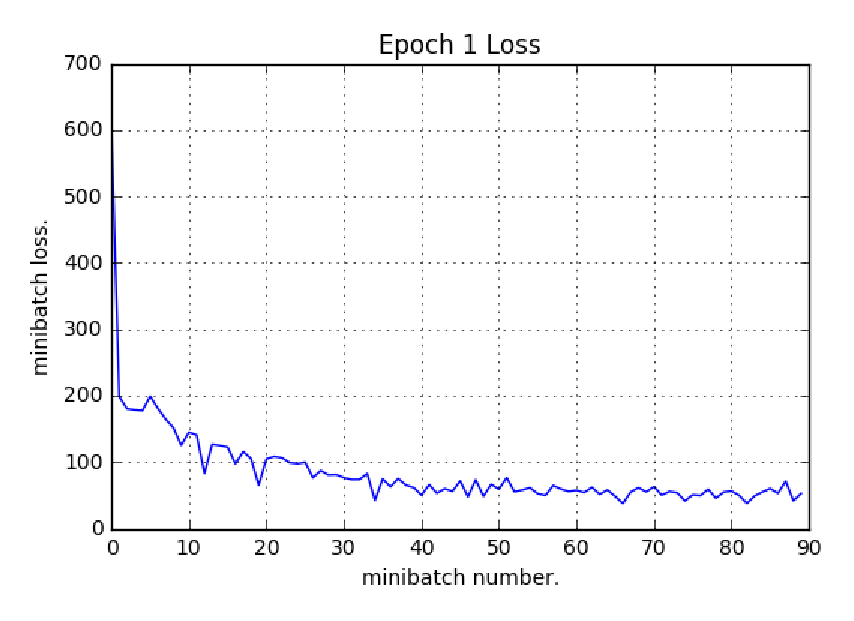
\epsfig{file=Figs4Paper/Plots/lossEpoch1.eps, height=1.5in, width=2.5in}
  \caption{Reduction in loss over several mini-batches in the first epoch}
  \label{fig:lossepoch1}
%  }
\end{figure}


Table~\ref{table:classificationresults} shows the accuracy metric for train, validation and test sets.

\begin{table}
\begin{center}
\begin{tabular}{|l|c|c|}
\hline
Dataset & Num of Images & Accuracy \\
\hline\hline
Train & 5756 & 0.18 \\
Validate & 1619 & 0.2 \\
Test & 819 & 0.0842 \\
\hline
\end{tabular}
\end{center}
\caption{Dataset Details}
\label{table:classificationresults}
\end{table}

\subsubsection{Discussion}
\label{subsubsec:pb1discussion}

We observe that train (and validate) accuracy is much higher than the test accuracy. This suggests that we are probably overfitting the training set. We plan to investigate this in depth going forward, including the use of (a) dropout (b)  L2 weight regularization  (c) increasing size of the dataset etc. Any feedback on how to improve the test accuracy is highly welcome.

\subsection{Detecting individual food items in an image.}

For this problem we are planning to use some standard CNN based detection methods such as SSD~\cite{liu2016ssd}, Fast-RCNN~\cite{ren2015faster} and YOLO~\cite{redmon2016you}. These approaches typically detect bounding boxes of interest in an image, and we want to leverage these techniques to detect the individual food items in an image. For this milestone we were not able to make much progress on this problem. We plan to work on this in the coming weeks. 


